\documentclass[journal,12pt,twocolumn]{IEEEtran}
\usepackage{setspace}
\usepackage{gensymb}
\singlespacing
\usepackage[cmex10]{amsmath}
\usepackage{amsthm}
\usepackage{mathrsfs}
\usepackage{txfonts}
\usepackage{stfloats}
\usepackage{bm}
\usepackage{cite}
\usepackage{cases}
\usepackage{subfig}
\usepackage{longtable}
\usepackage{multirow}
\usepackage{enumitem}
\usepackage{mathtools}
\usepackage{tikz}
\usepackage{circuitikz}
\usepackage{verbatim}
\usepackage[breaklinks=true]{hyperref}
\usepackage{tkz-euclide} % loads  TikZ and tkz-base
\usepackage{listings}
\usepackage{color}    
\usepackage{array}    
\usepackage{longtable}
\usepackage{calc}     
\usepackage{multirow} 
\usepackage{hhline}   
\usepackage{ifthen}   
\usepackage{lscape}     
\usepackage{chngcntr}
\DeclareMathOperator*{\Res}{Res}
\renewcommand\thesection{\arabic{section}}
\renewcommand\thesubsection{\thesection.\arabic{subsection}}
\renewcommand\thesubsubsection{\thesubsection.\arabic{subsubsection}}

\renewcommand\thesectiondis{\arabic{section}}
\renewcommand\thesubsectiondis{\thesectiondis.\arabic{subsection}}
\renewcommand\thesubsubsectiondis{\thesubsectiondis.\arabic{subsubsection}}
\renewcommand\thetable{\arabic{table}}
% correct bad hyphenation here
\hyphenation{op-tical net-works semi-conduc-tor}
\def\inputGnumericTable{}                                 %%

\lstset{
%language=C,
frame=single, 
breaklines=true,
columns=fullflexible
}
%\lstset{
%language=tex,
%frame=single, 
%breaklines=true
%}

\begin{document}
\newtheorem{theorem}{Theorem}[section]
\newtheorem{problem}{Problem}
\newtheorem{proposition}{Proposition}[section]
\newtheorem{lemma}{Lemma}[section]
\newtheorem{corollary}[theorem]{Corollary}
\newtheorem{example}{Example}[section]
\newtheorem{definition}[problem]{Definition}
\newcommand{\BEQA}{\begin{eqnarray}}
\newcommand{\EEQA}{\end{eqnarray}}
\newcommand{\define}{\stackrel{\triangle}{=}}
\bibliographystyle{IEEEtran}
\providecommand{\mbf}{\mathbf}
\providecommand{\pr}[1]{\ensuremath{\Pr\left(#1\right)}}
\providecommand{\tr}[1]{\ensuremath{\textrm{tr}\left(#1\right)}}
\providecommand{\qfunc}[1]{\ensuremath{Q\left(#1\right)}}
\providecommand{\sbrak}[1]{\ensuremath{{}\left[#1\right]}}
\providecommand{\lsbrak}[1]{\ensuremath{{}\left[#1\right.}}
\providecommand{\rsbrak}[1]{\ensuremath{{}\left.#1\right]}}
\providecommand{\brak}[1]{\ensuremath{\left(#1\right)}}
\providecommand{\lbrak}[1]{\ensuremath{\left(#1\right.}}
\providecommand{\rbrak}[1]{\ensuremath{\left.#1\right)}}
\providecommand{\cbrak}[1]{\ensuremath{\left\{#1\right\}}}
\providecommand{\lcbrak}[1]{\ensuremath{\left\{#1\right.}}
\providecommand{\rcbrak}[1]{\ensuremath{\left.#1\right\}}}
\theoremstyle{remark}
\newtheorem{rem}{Remark}
\newcommand{\sgn}{\mathop{\mathrm{sgn}}}
\providecommand{\abs}[1]{\left\vert#1\right\vert}
\providecommand{\res}[1]{\Res\displaylimits_{#1}} 
\providecommand{\norm}[1]{\left\lVert#1\right\rVert}
\providecommand{\mtx}[1]{\mathbf{#1}}
\providecommand{\mean}[1]{E\left[ #1 \right]}
\providecommand{\fourier}{\overset{\mathcal{F}}{ \rightleftharpoons}}
\providecommand{\system}[1]{\overset{\mathcal{#1}}{ \longleftrightarrow}}
\newcommand{\solution}{\noindent \textbf{Solution: }}
\newcommand{\cosec}{\,\text{cosec}\,}
\providecommand{\dec}[2]{\ensuremath{\overset{#1}{\underset{#2}{\gtrless}}}}
\newcommand{\myvec}[1]{\ensuremath{\begin{pmatrix}#1\end{pmatrix}}}
\newcommand{\mydet}[1]{\ensuremath{\begin{vmatrix}#1\end{vmatrix}}}
\let\vec\mathbf
\def\putbox#1#2#3{\makebox[0in][l]{\makebox[#1][l]{}\raisebox{\baselineskip}[0in][0in]{\raisebox{#2}[0in][0in]{#3}}}}
     \def\rightbox#1{\makebox[0in][r]{#1}}
     \def\centbox#1{\makebox[0in]{#1}}
     \def\topbox#1{\raisebox{-\baselineskip}[0in][0in]{#1}}
     \def\midbox#1{\raisebox{-0.5\baselineskip}[0in][0in]{#1}}

\vspace{3cm}
\title{Semidefinite Programming Assignment}
\author{Gautam Singh}
\maketitle
\bigskip

\begin{abstract}
    This document contains the solution to Question 21 of 
    Exercise 6 in Chapter 6 of the class 12 NCERT textbook.
\end{abstract}

\begin{enumerate}
    \item The line 
    \begin{align}
        y = mx + 1 \label{eq:line}
    \end{align}
    is a tangent to the curve
    \begin{align}
        y^2 = 4x \label{eq:curve}
    \end{align}
    if the value of $m$ is
    \begin{enumerate}
        \item 1
        \item 2
        \item 3
        \item $\frac{1}{2}$
    \end{enumerate}

    \solution Rewriting \eqref{eq:line} and \eqref{eq:curve} in standard forms,
    we get,
    \begin{align}
        \vec{n} = \myvec{m\\-1}, c = -1 \label{eq:line-params} \\
        \vec{V} = \myvec{0&0\\0&1}, \vec{u} = \myvec{-2\\0}, f = 0 \label{eq:curve-params}
    \end{align}
    Now, we rotate the axes by applying the transformation
    \begin{align}
        \vec{x} \leftarrow \vec{Px}
        \label{eq:trans}
    \end{align}
    such that
    \begin{align}
        \vec{Pn} = \vec{e_1} \label{eq:n-e1}
    \end{align}
    We find $\vec{P}$ by forming the augmented matrix
    \begin{align}
        \myvec{1&0&m\\0&1&-1} &\xleftrightarrow[]{R_1 \leftarrow \frac{R_1}{m}} \myvec{\frac{1}{m}&0&1\\0&1&-1} \\
                &\xleftrightarrow[]{R_2 \leftarrow R_1 + R_2} \myvec{\frac{1}{m}&0&1\\\frac{1}{m}&1&0}
                \label{eq:aug-P}
    \end{align}
    giving
    \begin{align}
        \vec{P} = \myvec{\frac{1}{m}&0\\\frac{1}{m}&1}
        \label{eq:P-val}
    \end{align}
    Thus, using \eqref{eq:trans}, the optimization problem becomes
    \begin{align}
        \min_{\vec{x}} \norm{\vec{x}}^2 \label{eq:cost} \\
        \textrm{s.t. } \vec{x}^\top\vec{P}^\top\vec{VPx} + 2\vec{u}^\top\vec{Px} + f = 0 \label{eq:constr}
    \end{align}
    We use semidefinite programming to solve this problem. Setting
    \begin{align}
        \vec{y} = \myvec{\vec{x}\\1}
    \end{align}
    we rewrite the optimization problem as
    \begin{align}
        \min_{\vec{y}}\vec{y}^\top\vec{Cy} \label{eq:y-cost} \\
        \textrm{s.t. } \vec{y}^\top\vec{Ay} = 0 \label{eq:y-constr}
    \end{align}
    Using semidefinite relaxation, the problem becomes
    \begin{align}
        \min_{\vec{Y}} \tr{\vec{CY}} \label{eq:sd-cost} \\
        \textrm{s.t. } \tr{\vec{AY}} = 0 \label{eq:sd-constr} \\
        \vec{A} \succeq \vec{0} \label{eq:sd-psd}
    \end{align}
    The Python code \texttt{codes/sdp.py} solves this problem by plotting
    the values of \eqref{eq:sd-cost} in Fig. \ref{fig:sdp-graph} and choosing 
    $m$ appropriately using \textit{cvxpy}. The cost \eqref{eq:sd-cost} is 
    minimized when $m = \pm 1$. Hence, option \textbf{a)} is correct.
    \begin{figure}[!ht]
        \centering
        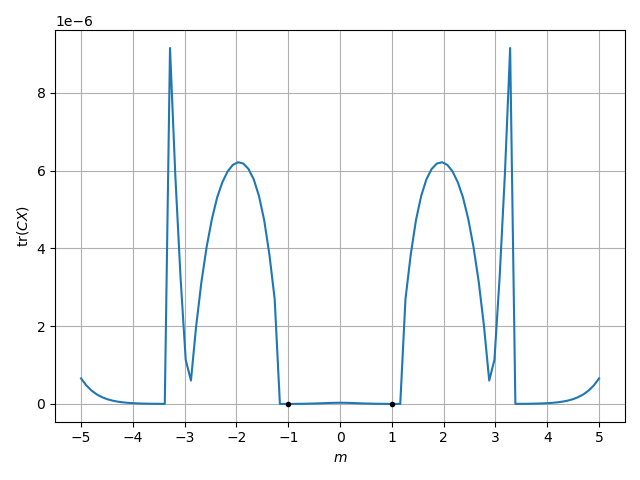
\includegraphics[width=\columnwidth]{figs/sdp.png}
        \caption{Cost for various values of $m$.}
        \label{fig:sdp-graph}
    \end{figure}
\end{enumerate}
\end{document}
